\documentclass[times, twocolumn]{zHenriquesLab-StyleBioRxiv}
%----------------------------------------------------------------------------------------
%	PACKAGES AND OTHER DOCUMENT CONFIGURATIONS
%----------------------------------------------------------------------------------------

\usepackage{amsmath, amsfonts, amsthm} % Math packages

% Packages for Title Page
% \usepackage{newlfont}
% \usepackage{gensymb}

% \usepackage{listings} % Code listings, with syntax highlighting

\usepackage[utf8]{inputenc}
% \usepackage[english,vietnam]{babel}
% \usepackage[utf7]{vietnam}

%----------------------------------------------------------------------------------------
%	IMAGES CONFIGURATION
%----------------------------------------------------------------------------------------
\usepackage{graphicx} % Required for inserting images
\graphicspath{{Figures/}{./}} % Specifies where to look for included images (trailing slash required)
\usepackage{xstring}

\usepackage{subcaption}
\DeclareCaptionFormat{custom}
{
    \normalsize\textit{#1}\textit{#2}\textit{\normalsize #3}
}
\captionsetup{format=custom}


%----------------------------------------------------------------------------------------
%	LIST CONFIGURATION
%----------------------------------------------------------------------------------------
% \usepackage{enumitem} % Required for list customisation
% \setlist{noitemsep} % No spacing between list items


%----------------------------------------------------------------------------------------
%	PARAGRAPH FORMATTING 
%----------------------------------------------------------------------------------------
% \setlength\parindent{0pt} % Removes all indentation from paragraphs
% \setlength{\parindent}{2em}
\usepackage{indentfirst}
% \usepackage[skip=10pt plus1pt, indent=25pt]{parskip}

%----------------------------------------------------------------------------------------
%	DOCUMENT MARGINS
%----------------------------------------------------------------------------------------
% \usepackage{geometry} % Required for adjusting page dimensions and margins

% \geometry{
% 	paper=a4paper, % Paper size, change to letterpaper for US letter size
% 	top=2cm, % Top margin
% 	bottom=2.5cm, % Bottom margin
% 	left=3cm, % Left margin
% 	right=3cm, % Right margin
% 	headheight=0.75cm, % Header height
% 	footskip=1.5cm, % Space from the bottom margin to the baseline of the footer
% 	headsep=0.75cm, % Space from the top margin to the baseline of the header
% 	%showframe, % Uncomment to show how the type block is set on the page
% }

%----------------------------------------------------------------------------------------
%	FONTS
%----------------------------------------------------------------------------------------
% \usepackage[utf8]{inputenc} % Required for inputting international characters
% \usepackage[T1]{fontenc} % Use 8-bit encoding
% \usepackage{fourier} % Use the Adobe Utopia font for the document
% \usepackage{sectsty}
\usepackage[usenames,dvipsnames]{color}
% \sectionfont{\fontsize{12}{22}\selectfont}

%----------------------------------------------------------------------------------------
%	SECTION 
%----------------------------------------------------------------------------------------
% \setcounter{section}{14}
% \usepackage{sectsty} % Allows customising section commands

% \sectionfont{\vspace{6pt}\centering\normalfont\scshape} % \section{} styling
% \subsectionfont{\normalfont\bfseries} % \subsection{} styling
% \subsubsectionfont{\normalfont\itshape} % \subsubsection{} styling
% \paragraphfont{\normalfont\scshape} % \paragraph{} styling

%----------------------------------------------------------------------------------------
%	HEADERS AND FOOTERS
%----------------------------------------------------------------------------------------
% \usepackage{scrlayer-scrpage} % Required for customising headers and footers

% \ohead*{} % Right header
% \ihead*{} % Left header
% \chead*{} % Centre header

% \ofoot*{} % Right footer
% \ifoot*{} % Left footer
% \cfoot*{} % Centre footer
 % Include the file specifying the document structure and custom commands
\usepackage[utf8]{vietnam}
\usepackage{multicol}
% Please give the surname of the lead author for the running footer
\leadauthor{Ze Liu} 

\begin{document}

\title{Swin Transformer V2: Cải thiện Năng lực và Độ phân giải}

% Use letters for affiliations, numbers to show equal authorship (if applicable) and to indicate the corresponding author
\author{Ze Liu \hspace{5pt} Han Hu \hspace{5pt} Yutong Lin \hspace{5pt} Zhuliang Yao \hspace{5pt} Zhenda Xie \hspace{5pt} Yixuan Wei \hspace{5pt} Jia Ning \\ Yue Cao \hspace{5pt} Zheng Zhang \hspace{5pt} Li Dong \hspace{5pt} Furu Wei \hspace{5pt} Baining Guo}

\affil{Microsoft Research Asia}

\maketitle

\begin{center}
    \bfseries\large{Tóm tắt}
\end{center}
\begin{abstract}

Chúng tôi trình bày các kỹ thuật mở rộng Swin Transformer lên đến 3 tỷ tham số và có khả năng huấn luyện với những hình ảnh có độ phân giải lên đến $1.536 \times 1.536$ điểm ảnh. Bằng cách mở rộng năng lực và độ phân giải, Swin Transformer thiết lập các kỷ lục mới trên các thang đánh giá đại diện cho bốn bài toán thị giác máy tính: độ chính xác $top-1$ cho bài tóan phân loại hình ảnh ImageNet-V2 là $84,0\%$, baì toán phát hiện vật thể COCO là $63,1/54,4 box/mask mAP$, bài toán phân đoạn ngữ nghĩa (\textit{semantic segmentation}) ADE20K là $59,9 mIoU$, và độ chính xác $top-1$ cho bài toán phân loại hành động trong video Kinetics-400 là $86,8\%$.

Chúng tôi giải quyết các vấn đề về tính không ổn định trong huấn luyện mô hình và nghiên cứu cách chuyển đổi hiệu quả các mô hình được tiền huấn luyện ở độ phân giải thấp sang các mô hình có độ phân giải cao hơn. Với mục tiêu này, một số kỹ thuật mới được đề xuất: $1)$ Kỹ thuật phần dư sau chuẩn hóa và phương pháp tiếp cận tập trung cosine mở rộng (\textit{scaled cosine attention}) để cải thiện tính ổn định của các mô hình thị giác lớn; $2)$ Kỹ thuật chệch vị liên tục không gian log (log-spaced continuous position bias) để chuyển đổi một cách hiệu quả các mô hình tiền huấn luyện với hình ảnh và khẩu độ (\textit{window}) ở độ phân giải thấp sang các hình ảnh và khẩu độ có độ phân giải cao hơn.

Ngoài ra, chúng tôi cũng chia sẻ các chi tiết quan trọng khi triển khai giúp tiết kiệm đáng kể mức tiêu thụ bộ nhớ GPU và do đó, việc huấn luyện các mô hình thị giác lớn bằng GPU thông thường trở nên khả thi. Sử dụng các kỹ thuật này và việc tiền huấn luyện có giám sát, chúng tôi đã huấn luyện thành công mô hình Swin Transformer với 3 tỷ tham số và sử dụng nó cho nhiều bài toán thị giác khác nhau trên các hình ảnh và khẩu độ có độ phân giải cao, đạt được độ chính xác tốt nhất hiện nay (state of the art) trên nhiều thang đánh giá khác nhau. Code có tại đường dẫn \textcolor{red}{https://github.com/microsoft/Swin-Transformer}.
\end {abstract}

\section*{1. Giới thiệu}
Việc mở rộng các mô hình ngôn ngữ đã chứng kiến sự thành công ngoài sức mong đợi. Năng lực của các mô hình có sự cải thiện đáng kể trên các bài toán ngôn ngữ và thể hiện khả năng học từ ít dữ liệu hơn tương tự như con người. Kể từ mô hình lớn BERT với $340$ triệu tham số, các mô hình ngôn ngữ nhanh chóng được mở rộng hơn $1.000$ lần chỉ trong vài năm, đạt tới $530$ tỷ tham số đặc và $1.6$ nghìn tỷ tham số thưa. Các mô hình ngôn ngữ lớn này cũng được cho là có khả năng xử lý mạnh mẽ từ ít dữ liệu trên nhiều bài toán xử lý ngôn ngữ khác nhau giống như trí thông minh của con người.

\begin{figure}[!ht] % [!ht] forces the figure to be output where it is defined in the code (it suppresses floating)
    \centering
    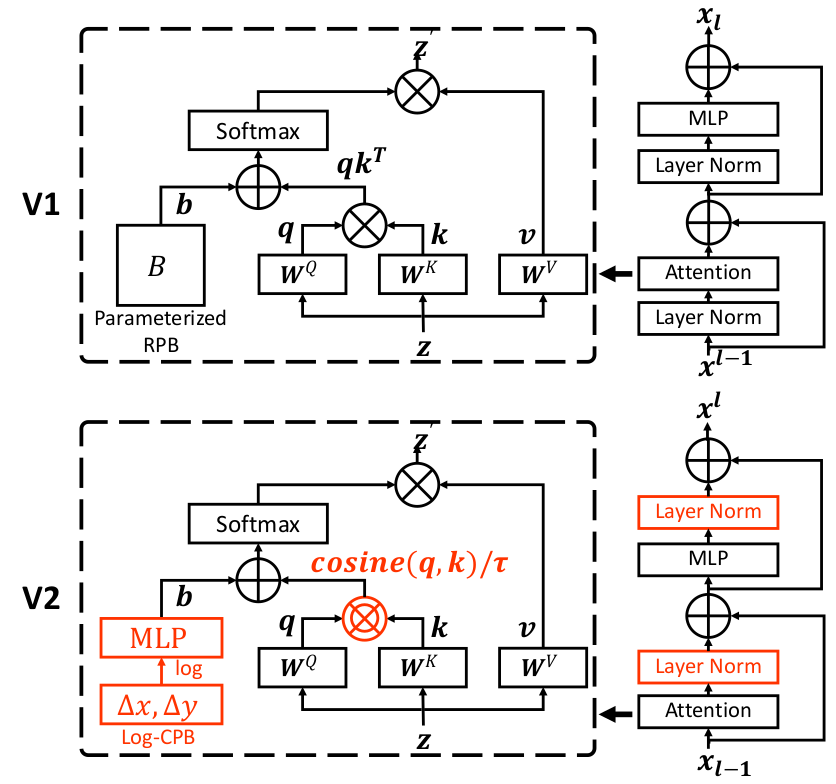
\includegraphics[width=1\columnwidth]{1.png}
    \caption{Để mở rộng tốt hơn năng lực và độ phân giải của mô hình, một số điều chỉnh được thực hiện trên kiến trúc Swin Transformer ban đầu (V1): 1) Một res-post-norm thay thế cấu hình pre-norm trước đó; 2) \textit{Scaled cosine attention} thay thế các tiếp cận dot product attention ban đầu; 3) Phương pháp tiếp cận log-spaced continuous relative position bias thay thế cách tiếp cận tham số hóa trước đây. Phương pháp 1) và 2) giúp mô hình mở rộng năng lực dễ dàng hơn. Phương pháp 3) giúp mô hình chuyển đổi tốt hơn với các độ phân giải khẩu độ khác nhau. Kiến trúc được cải thiện này gọi là Swin Transformer V2.}
\end{figure}

Mặt khác, việc mở rộng quy mô của các mô hình thị giác đã bị tụt hậu. Mặc dù từ lâu người ta đã nhận ra rằng các mô hình thị giác lớn hơn thường thực hiện tốt hơn, nhưng kích thước tuyệt đối của các mô hình gần đây nhất mới chỉ có thể đạt khoảng $1-2$ tỷ tham số. Quan trọng hơn, không giống như các mô hình ngôn ngữ lớn, các mô hình thị giác lớn hiện có chỉ được áp dụng cho việc phân loại hình ảnh.

Để huấn luyện thành công mô hình thị giác tổng quát và lớn, chúng ta cần giải quyết một số vấn đề chính. Thứ nhất, các thử nghiệm của chúng tôi với các mô hình thị giác lớn cho thấy tính không ổn định trong huấn luyện. Chúng tôi thấy rằng sự khác biệt về biên độ hoạt hóa giữa các lớp trở nên lớn hơn đáng kể trong các mô hình lớn. Xem xét kỹ hơn kiến trúc ban đầu cho thấy điều này là do đầu ra của đơn vị dư (\textit{residual unit}) được thêm trực tiếp vào nhánh chính. Kết quả là các giá trị kích hoạt được tích lũy theo từng lớp, và do đó biên độ ở các lớp sâu hơn lớn hơn đáng kể so với các biên độ ở các lớp ban đầu. Để giải quyết vấn đề này, chúng tôi đề xuất một cấu hình chuẩn hóa mới, được gọi là res-post-norm, chuyển lớp LN từ phần đầu của \textit{residual unit} ra phía sau, như trong Hình 1. Chúng tôi nhận thấy cấu hình mới này tạo ra các giá trị kích hoạt nhẹ hơn nhiều trên các lớp mạng. Chúng tôi cũng đề xuất cách tiếp cận \textit{scaled cosine attention} thay thế dot product attention trước đó. \textit{scaled cosine attention} làm cho việc tính toán không liên quan đến biên độ đầu vào khối, và các giá trị attention ít có khả năng rơi vào các giá trị cực trị. Trong các thí nghiệm của chúng tôi, hai kỹ thuật được đề xuất không chỉ giúp quá trình huấn luyện ổn định hơn mà còn cải thiện độ chính xác, đặc biệt là đối với các mô hình lớn hơn.

Thứ hai, nhiều tác vụ thị giác xuôi như phát hiện vật thể và phân đoạn ngữ nghĩa yêu cầu hình ảnh đầu vào có độ phân giải cao hoặc khẩu độ attention lớn. Sự biến thiên của kích thước khẩu độ giữa tiền huấn luyện độ phân giải thấp và tinh chỉnh (\textit{fine-tune}) độ phân giải cao có thể khá lớn. Phổ biến hiện nay là thực hiện phép nội suy hai khối (\textit{bi-cubic interpolation}) của các ánh xạ chệch vị (\textit{position bias map}). Cách khắc phục đơn giản này khá đặc biệt và kết quả thường là chưa tối ưu. Chúng tôi giới thiệu hướng tiếp cận chệch vị liên tục không gian log (Log-CPB), giúp sinh ra các giá trị chệch vị đối với các khoảng tọa độ tùy ý bằng cách áp dụng một mạng meta nhỏ với đầu vào là tọa độ dạng không gian log. Vì mạng meta lấy bất kỳ tọa độ nào, nên một mô hình tiền huấn luyện sẽ có thể tự do chuyển qua các khẩu độ bằng cách chia sẻ trọng số của mạng meta. Một thiết kế quan trọng trong cách tiếp cận của chúng tôi là chuyển đổi các tọa độ sang không gian log để tỷ lệ ngoại suy có thể thấp ngay cả khi khẩu độ mục tiêu lớn hơn đáng kể so với khẩu độ tiền huấn luyện. Việc mở rộng năng lực và độ phân giải của mô hình cũng dẫn đến mức tiêu thụ bộ nhớ GPU rất cao so với các mô hình thị giác hiện có. Để giải quyết vấn đề về bộ nhớ, chúng tôi kết hợp một số kỹ thuật quan trọng bao gồm zero-optimizer, con trỏ kiểm tra kích hoạt (activation check pointing) và tính toán self-attention tuần tự. Với các kỹ thuật này, mức tiêu thụ bộ nhớ GPU của các mô hình lớn và độ phân giải cao giảm đáng kể trong khi chỉ giảm một chút về tốc độ huấn luyện.

Với các kỹ thuật trên, chúng tôi đã huấn luyện thành công mô hình Swin Transformer với 3 tỷ tham số và áp dụng hiệu quả sang các bài toán thị giác khác nhau với độ phân giải hình ảnh lớn tới $1.536 \times 1.536$ điểm ảnh, sử dụng GPU Nvidia A100-40G. Trong xử lý mô hình tiền huấn luyện, chúng tôi cũng sử dụng tiền huấn luyện tự giám sát để giảm sự phụ thuộc vào lượng lớn dữ liệu gắn nhãn. Với dữ liệu được dán nhãn ít hơn 40 lần so với cách tiếp cận trước đây (JFT-3B), mô hình với 3 tỷ tham số đạt được độ chính xác cao nhất trên một loạt thang đánh giá các bài toán thị giác. Cụ thể, nó đạt được độ chính xác $top-1$ cho bài toán phân loại hình ảnh trên tập ImageNet-V2 là $84,0$, phát hiện vật thể trên tập COCO là $63,1/54,4 box/mask mAP$, phân đoạn ngữ nghĩa trên tập ADE20K là $59,9 mIoU$, và độ chính xác $top-1$ phân loại hành động trong video Kinetics-400 là $86,8\%$, cao hơn $+ NA\%, + 4,4 / + 3,3, +6,3$ và $+1,9$ so với các con số tốt nhất trong Swin Transformers ban đầu và vượt qua kỷ lục trước đó tương ứng là $+ 0,8\%, + 1,8 / + 1,4, +1,5$ và $+ 1,4\%$.

Bằng cách mở rộng cả năng lực và độ phân giải của các mô hình thị giác với hiệu suất cao trên các bài toán thị giác thông thường, giống như hiệu suất của mô hình trên các bài toán xử lý ngôn ngữ tự nhiên, chúng tôi mong muốn tiến hành nhiều nghiên cứu theo hướng này hơn để có thể thu hẹp khoảng cách giữa mô hình thị giác và các mô hình ngôn ngữ và tạo điều kiện thuận lợi cho việc tạo mô hình chung của hai lĩnh vực.

\section*{2. Các công trình nghiên cứu có liên quan}

\textbf{Các mạng ngôn ngữ và mở rộng} Các công trình tiên phong về Transformer được xem là các mạng tiêu chuẩn. Việc khám phá mở rộng năng lực của kiến trúc này đã bắt đầu được đẩy nhanh nhờ việc phát minh ra các phương pháp học tự giám sát, chẳng hạn như mô hình ngôn ngữ có mặt nạ (\textit{masked}) hay tự động hồi quy (\textit{auto-regressive}), và đã được đẩy mạnh hơn bởi quy luật mở rộng. Kể từ đó, năng lực của các mô hình ngôn ngữ đã tăng đáng kể, lên tới hơn 1.000 lần trong vài năm, từ BERT-340M đến Megatron-Turing-530B và Switch-Transformer-1.6T tham số thưa. Với kích thước tăng, độ chính xác trên các thang đánh giá về ngôn ngữ khác nhau đã được cải thiện đáng kể. Hiệu suất \textit{zero-shot} hoặc \textit{few-shot} cũng được cải thiện đáng kể, đây là nền tảng của trí tuệ con người.

\vspace*{5mm}
\textbf{Mạng thị giác và mở rộng} CNN từ lâu đã trở thành mạng thị giác máy tính tiêu chuẩn. Kể từ AlexNet, các kiến trúc ngày càng trở nên sâu hơn và lớn hơn, điều này đã cải thiện rất nhiều các bài toán thị giác khác nhau và thúc đẩy làn sóng học sâu trong thị giác máy tính, chẳng hạn như VGG, GoogleNet và ResNet. Trong hai năm qua, kiến trúc CNN đã được mở rộng hơn nữa lên khoảng 1 tỷ tham số, tuy nhiên, hiệu suất tuyệt đối có sự cải thiện không đáng kể, có lẽ do thiên hướng quy nạp trong kiến trúc CNN đã hạn chế sức mạnh của mô hình.

\vspace*{5mm}
Năm ngoái, Transformers đã lần lượt dẫn đầu các thang đánh giá thị giác, bao gồm phân loại hình ảnh trên tập ImageNet-1K, phát hiện vật thể trên tập COCO, phân đoạn ngữ nghĩa trên tập ADE20K, phân loại video trên tập Kinetics-400, v.v. Kể từ những công trình này, nhiều biến thể Transformer cho lĩnh vực thị giác đã được đề xuất nhưng độ chính xác chỉ được cải thiện ở quy mô tương đối nhỏ. Chỉ có một số công trình cố gắng mở rộng năng lực của mô hình Transformers thị giác. Tuy nhiên, chúng cần số lượng lớn dữ liệu ảnh được gán nhãn, ví dụ như JFT-3B, và chỉ được áp dụng cho các bài toán phân loại hình ảnh.

\vspace*{5mm}
\textbf{Chuyển tiếp giữa các khẩu độ / độ phân giải nhân (kernel) khác nhau} Đối với CNN, các công trình trước đây thường cố định kích thước nhân (\textit{kernel}) trong quá trình tiền huấn luyện và tinh chỉnh. Các Transformer thị giác toàn cục, như ViT, tính toán \textit{attention} toàn cục, với khẩu độ \textit{attention} tỷ lệ thuận với độ phân giải ảnh đầu vào. Đối với kiến trúc Transformer thị giác cục bộ, chẳng hạn Transformer Swin, khẩu độ có thể được cố định hoặc thay đổi trong quá trình tinh chỉnh. Việc cho phép khẩu độ thay đổi sẽ thuận tiện hơn khi sử dụng, để có thể rải đều trên toàn bộ \textit{feature map} và điều chỉnh các trường tiếp nhận để có độ chính xác tốt hơn. Để xử lý các khẩu độ thay đổi giữa tiền huấn luyện và tinh chỉnh, nội suy hai khối là phương pháp phổ biến trước đây. Trong bài báo này, chúng tôi đề xuất cách tiếp cận chệch vị liên tục không gian log (Log-CPB) để áp dụng các trọng số từ mô hình tiền huấn luyện độ phân giải thấp sang các khẩu độ có độ phân giải cao hơn.

\vspace*{5mm}
\textbf{Nghiên cứu về các giá trị chệch (bias terms)} Trong NLP, phương pháp chệch vị tương đối (\textit{relative position bias}) tỏ ra có ích, so với phương pháp nhúng vị tuyệt đối (absolute position embedding) được sử dụng trong Transformer ban đầu. Trong thị giác máy tính, phương pháp chệch vị tương đối được sử dụng phổ biến hơn, có lẽ bởi vì các mối quan hệ không gian của tín hiệu thị giác đóng một vai trò quan trọng hơn trong mô hình thị giác. Một cách tiếp cận phổ biến là học trực tiếp các giá trị chệch dưới dạng trọng số của mô hình. Cũng có một số công trình tập trung nghiên cứu cách thiết lập và học các giá trị chệch.

\vspace*{5mm}
\textbf{Tích chập liên tục và các biến thể} Cách tiếp cận Log-CPB của chúng tôi cũng liên quan đến các công trình trước đây về tích chập liên tục và các biến thể, sử dụng mạng \textit{meta} để xử lý các điểm dữ liệu bất quy tắc. Phương pháp Log-CPB của chúng tôi được truyền cảm hứng từ những nỗ lực trong khi giải quyết một vấn đề khác là áp dụng các chệch vị tương đối trong Transformer thị giác với các khẩu độ tùy ý. Chúng tôi cũng đề xuất các tọa độ không gian log (\textit{log-spaced coordinates}) để giảm bớt khó khăn trong việc ngoại suy khi áp dụng giữa các thay đổi kích thước lớn.

\section*{3. Swin Transformer V2}
\subsection*{3.1. Khái quát về Swin Transformer}
Swin Transformer là xương sống cho nhiều bài toán thị giác máy tính và đã đạt được hiệu năng tốt trong các bài toán nhận dạng chi tiết như phát hiện vật thể cấp vùng ảnh, phân đoạn ngữ nghĩa cấp điểm ảnh và phân loại hình ảnh theo cấp độ hình ảnh. Ý tưởng chính của Swin Transformer là đưa một số tiền đề thị giác (\textit{visual priors}) quan trọng vào bộ mã hóa (\textit{encoder}) Transformer, bao gồm hệ thống phân cấp, địa phương và bất biến dịch, trong đó kết hợp sức mạnh của: đơn vị Transformer cơ bản có khả năng mô hình hóa mạnh và các tiền đề thị giác giúp mô hình dễ dàng ứng dụng cho các bài toán thị giác khác nhau.

\vspace*{5mm}
\textbf{Cấu hình chuẩn hóa (\textit{Normalization configuration})} Các kỹ thuật chuẩn hóa rất quan trọng trong việc huấn luyện một cách ổn định các mô hình có kiến trúc sâu. Swin Transformer ban đầu kế thừa kỹ thuật từ các mô hình Transformer ngôn ngữ và ViT để cấu hình chuẩn hóa trước mà không cần nghiên cứu sâu, như trong hình 1. Trong các phần mục nhỏ sau, chúng ta sẽ xem xét cấu hình chuẩn hóa mặc định này.

\vspace*{5mm}
\textbf{Độ chệch vị tương đối (\text{Relative position bias})} là một thành phần quan trọng trong Swin Transformer đời đầu, nó đưa ra một thuật ngữ chệch tham số bổ sung để mã hóa mối quan hệ hình học trong tính toán tự tập trung (\textit{self-attention}):

$$Attention(Q, K, V) = SoftMax(QK^{T} /\sqrt{d} + B)V, (1)$$

Trong đó $B \in R^{M^{2} \times M^{2}}$ là số hạng chệch vị tương đối cho mỗi đầu; $Q, K, V \in R^{M^{2} \times d}$ là các ma trận truy vấn \textit{query}, khóa \textit{key} và giá trị \textit{value}; $d$ là số chiều của $query/key$ và $M^{2}$ là số ô trong một khung. Độ chệch vị tương đối mã hóa các cấu hình không gian tương đối của các yếu tố thị giác và đóng vai trò quan trọng trong nhiều bài toán thị giác, đặc biệt đối với các bài toàn nhận dạng như phát hiện vật thể.

Trong Transformer Swin, các vị trí tương đối dọc theo mỗi trục nằm trong khoảng $[−M + 1, M - 1]$ và độ chệch vị tương đối được tham số hóa dưới dạng ma trận chệch $\hat{B} \in R^{(2M − 1) \times (2M − 1)}$, và các phần tử trong $B$ được lấy từ $\hat{B}$. Khi chuyển qua các khẩu độ khác nhau, ma trận chệch vị tương đối trong khóa tiền huấn luyện được sử dụng để khởi tạo ma trận chệch có kích thước khác nhau trong tinh chỉnh bằng nội suy hai khối.


\begin{figure}[!ht] % [!ht] forces the figure to be output where it is defined in the code (it suppresses floating)
    \centering
    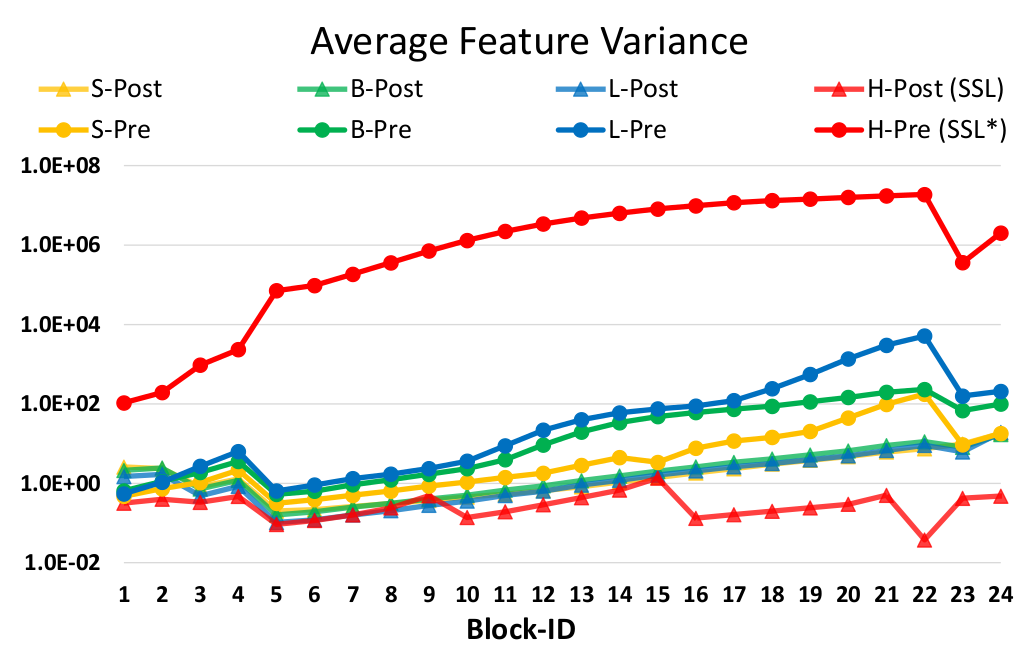
\includegraphics[width=1\columnwidth]{2.png}
    \caption{Biểu đồ lan truyền tín hiệu với các kích thước mô hình khác nhau. Các mô hình kích thước H được huấn luyện ở giai đoạn học tự giám sát và các kích thước khác được huấn luyện bằng nhiệm vụ phân loại ảnh. * cho thấy mô hình 40-epoch được sử dụng trước khi gặp sự cố.}
\end{figure}

\vspace*{5mm}
\textbf{Các vấn đề trong việc mở rộng mô hình và độ phân giải} Chúng tôi quan sát thấy hai vấn đề khi mở rộng quy mô và độ phân giả của Transformer Swin.

\vspace*{2mm}
• \textit{Một là tính không ổn định khi mở rộng năng lực mô hình}. Như trong Hình 2, khi chúng tôi mở rộng mô hình Swin Transformer ban đầu từ kích thước nhỏ sang kích thước lớn, các giá trị kích hoạt ở các lớp sâu hơn sẽ tăng lên đáng kể. Sự khác biệt giữa các lớp có biên độ cao nhất và thấp nhất đã đạt đến giá trị cực đại là $104$. Khi chúng tôi mở rộng nó lên một kích thước khổng lồ ($658$ triệu tham số), nó không thể hoàn thành quá trình huấn luyện, như thể hiện trong Hình 3.

\vspace*{2mm}
• \textit{Hiệu suất bị giảm sút khi áp dụng các mô hình giữa những độ phân giải khẩu độ khác nhau}. Trong hàng đầu tiên Bảng 1, độ chính xác giảm đáng kể khi chúng tôi trực tiếp kiểm tra độ chính xác của mô hình trên tập ImageNet-1K được tiền huấn luyện (ảnh $256 \times 256$ với khẩu độ $8 \times 8$) ở độ phân giải hình ảnh và khẩu độ lớn hơn thông qua phương pháp nội suy hai khối. Có thể cần kiểm tra lại cách tiếp cận chệch vị tương đối trong Swin Transformer ban đầu.
Trong các mục sau, chúng tôi trình bày các kỹ thuật giải quyết những vấn đề này, bao gồm hậu chuẩn hóa phần dư và \textit{scaled cosine attention} để giải quyết vấn đề không ổn định và phương pháp tiếp cận chệch vị liên tục không gian log để giải quyết vấn đề áp dụng giữa các độ phân giải khẩu độ khác nhau.

\begin{figure}[!ht] % [!ht] forces the figure to be output where it is defined in the code (it suppresses floating)
    \centering
    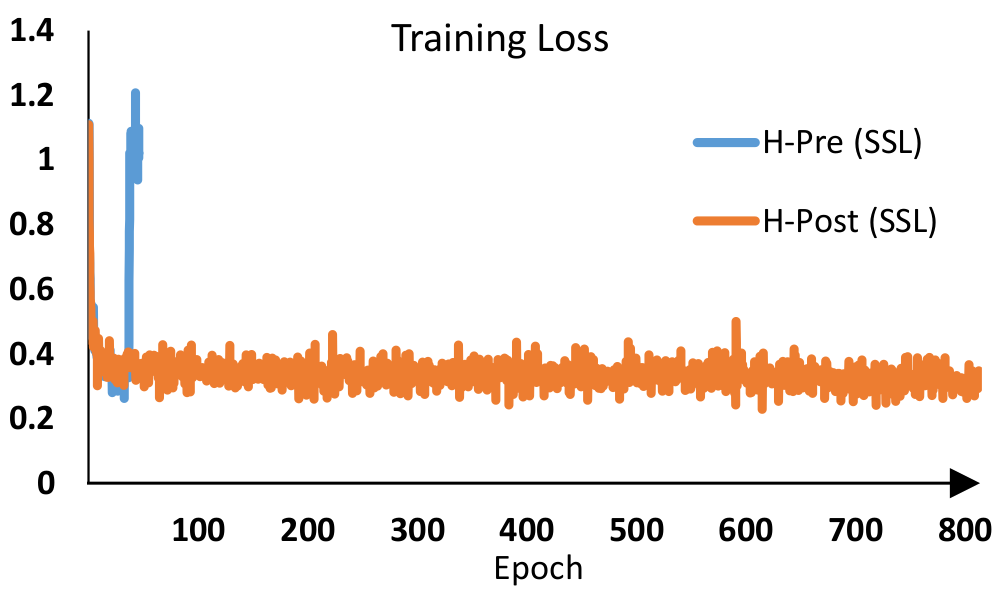
\includegraphics[width=1\columnwidth]{3.png}
    \caption{SwinV1-H so với SwinV2-H trong huấn luyện.}
\end{figure}

\subsection*{3.2. Mở rộng mô hình}
Như đã đề cập trong Phần 3.1, Transformer Swin ban đầu (và hầu hết các Transformer thị giác) sử dụng một lớp chuẩn hóa ở đầu mỗi khối, kế thừa từ mô hình ViT. Khi mở rộng mô hình, sự gia tăng đáng kể giá trị kích hoạt được quan sát thấy ở các lớp sâu hơn. Trên thực tế, trong cấu hình tiền chuẩn hóa, các giá trị kích hoạt đầu ra của mỗi khối dư được hợp nhất trực tiếp trở lại nhánh chính, và biên độ của nhánh chính ngày càng lớn hơn ở các lớp sâu hơn. Sự chênh lệch biên độ lớn ở các lớp khác nhau gây ra sự mất ổn định trong quá trình huấn luyện.

\vspace*{5mm}
\textbf{Hậu chuẩn hóa} Để giải quyết vấn đề này, chúng tôi đề xuất sử dụng phương pháp dư hậu chuẩn hóa (residual post normalization), như Hình 1. Trong cách tiếp cận này, đầu ra của mỗi khối dư được chuẩn hóa trước khi hợp nhất trở lại nhánh chính và biên độ của nhánh chính không cộng dồn khi xuống lớp sâu hơn. Như trong Hình 2, biên độ kích hoạt theo cách tiếp cận này nhẹ hơn nhiều so với cấu hình tiền chuẩn hóa như ban đầu.

Trong quá trình huấn luyện mô hình lớn nhất, chúng tôi giới thiệu một lớp chuẩn hóa lớp bổ sung trên nhánh chính cứ sau $6$ khối Transformer, để ổn định hơn nữa quá trình huấn luyện.

\vspace*{5mm}
\textbf{Scaled cosine attention} Trong tính toán self-attention ban đầu, các số hạng tương tự của các cặp pixel được tính như một tích giữa các vector \textit{query} và \textit{key}. Chúng tôi thấy rằng khi cách tiếp cận này được sử dụng trong các mô hình trực quan lớn, các ánh xá tập trung đã học của một số khối và phần đầu thường bị chi phối bởi một vài cặp pixel, đặc biệt là trong cấu hình res-post-norm. Để giải quyết vấn đề này, chúng tôi đề xuất một phương pháp tiếp cận \textit{scaled cosine attention} tính toán logit attention của một cặp pixel \textit{i} và \textit{j} bằng một hàm cosine:

$$Sim(q_{i}, k_{j}) = cos(q_{i}, k_{j})/\tau + B_{ij}, (2)$$

Trong đó $B_{ij}$ là độ lệch vị trí tương đối giữa pixel $i$ và $j$; $\tau$ là một đại lượng vô hướng có thể học được, không chia sẻ trên các lớp và các đầu. $\tau$ được đặt lớn hơn $0,01$. Hàm cosine được chuẩn hóa một cách tự nhiên và do đó có thể có các giá trị attention nhẹ hơn.

\subsection*{3.3. Mở rộng độ phân giải của khẩu độ}
Trong phần này, chúng tôi giới thiệu hướng tiếp cận chệch vị liên tục không gian log, để cho chệch vị liên tục có thể được chuyển đổi trơn tru theo các độ phân giải của khẩu độ.

\vspace*{5mm}
\textbf{Chệch vị tương đối liên tục} Thay vì trực tiếp tối ưu các \textit{bias} được tham số hóa, phương pháp tiếp cận chệch vị tương đối liên tục \textit{continuous relative position bias} sử dụng một mạng meta trên các tọa độ tương đối:

$$B(\Delta{x},\Delta{y}) = \mathcal{G}(\Delta{x},\Delta{y})$$

Với $\mathcal{G}$ là một mạng nhỏ, ví dụ một mạng MLP $2$ lớp với một hàm kích hoạt ReLU mặc định ở giữa.

Mạng $\mathcal{G}$ sinh ra các giá trị bias cho các tọa độ tương đối tùy ý, và vì vậy có thể được áp dụng một cách tự nhiên để tinh chỉnh các bài toán với kích thước khẩu độ thay đổi tùy ý. Trong khi suy diễn, các giá trị chệch ở mỗi vị trí tương đối có thể được tính toán trước và lưu lại như các tham số của mô hình, như vậy suy diễn cũng giống như cách tiếp cận giá trị chệch được tham số hóa ban đầu.

\vspace*{5mm}
\textbf{Các tọa độ không gian logarit} Khi áp dụng theo các kích thước khẩu độ thay đổi lớn, phần lớn khoảng tọa độ tương đối cần phải được ngoại suy. Để giảm nhẹ vấn đề này, chúng tôi đề xuất sử dụng các tọa độ không gian logarit thay vì không gian tuyến tính như lúc đầu:

$$
    \begin{aligned}
        \widehat{\Delta{x}} = sign(x).log(1+|\Delta{x}|), \\
        \widehat{\Delta{y}} = sign(y).log(1+|\Delta{y}|),
    \end{aligned}
$$

Với $\Delta{x}$, $\Delta{y}$ và $\widehat{\Delta{x}}$ ,$\widehat{\Delta{y}}$ là các tọa độ tương ứng ở không gian log và được mở rộng tuyến tính.

Bằng việc sử dụng các tọa độ không gian log, khi ta chuyển đổi các chệch vị tương đối theo các độ phân giải của khẩu độ, tỉ lệ ngoại suy yêu cầu sẽ nhỏ hơn giá trị chệch mà sử dụng tọa độ không gian tuyến tính ban đầu. Lấy ví dụ chuyển đổi từ kích thước khẩu độ $8 \times 8$ được tiền huấn luyện sang một kích thước khẩu độ $16\times16$ đã được tinh chỉnh, sử dụng các tọa độ gốc ban đầu, khoảng tọa độ đầu vào sẽ là từ $[-7,7]\times[-7,7]$ tới $[-15,15]\times[-15,15]$.

Tỉ lệ ngoại suy là $8/7=1.14 \times$ khoảng ban đầu. Sử dụng các tọa độ không gian log, khoảng đầu vào sẽ từ $[-1.079,2.079] \times [-2.079,2.0790]$ tới $[-2.773,2.773]\times[-2.773,2.773]$. Tỉ lệ ngoại suy là $0.33\times$ khoảng ban đầu, tức là nhỏ hơn khoảng $4$ lần tỉ lệ ngoại suy sử dụng tọa độ không gian tuyến tính ban đầu.

Bảng 1 so sánh hiệu năng chuyển đổi của các hướng tính toán khác nhau giá trị chệch vị. Có thể thấy rằng hướng tiếp cận chệch vị liên tục không gian log (log-spaced CPB) cho hiệu năng tốt nhất, đặc biệt khi được chuyển đổi sang các kích thước khẩu độ lớn hơn.

\subsection*{3.4. Tiền huấn luyện tự giám sát}

Các mô hình lớn hơn thì cũng cần nhiều dữ liệu hơn. Để giải quyết vấn đề cần nhiều dữ liệu, các mô hình thị giác lớn điển hình trước đây khai thác các tập dữ liệu có nhãn lớn như JFT-3B. Trong bài báo này, chúng tôi vận dụng phương pháp tiền huấn luyện tự giám sát, SimMIM, để giải quyết yêu cầu cần dữ liệu có nhãn. Bằng cách này, chúng tôi đã huấn luyện thành công mô hình Swin Transformer mạnh mẽ với $3$ tỷ tham số và đạt được kết quả SOTA trên 4 tập đánh giá đại diện, với chỉ $70$ triệu ảnh có nhãn (bằng $1/40$ tập JFT-3B).


\subsection*{3.5. Cách triển khai để tiết kiệm bộ nhớ GPU}

Một vấn đề khác nằm ở việc sử dụng bộ nhớ GPU khá tốn kém với cách triển khai thông thường khi cả năng lực và độ phân giải đều lớn. Để giải quyết vấn đề về bộ nhớ, chúng tôi áp dụng các kỹ thuật sau:

\begin{itemize}
    \item \textit{Hàm tối ưu không dư (Zero-redundancy Optimizer)(ZeRO)}. Trong cách triển khai các hàm tối ưu song song hóa dữ liệu, các tham số mô hình và trạng thái tối ưu được truyền trực tiếp tới mỗi GPU. Cách triển khai này rất ko phù hợp trong việc sử dụng bộ nhớ GPU, ví dụ, một mô hình với $3$ tỉ tham số sẽ tiêu tốn $46GB$ bộ nhớ GPU khi một hàm tối ưu AdamW và kiểu dữ liệu $fp32$ được sử dụng. Với một hàm tối ưu ZeRO, các tham số của mô hình và các trạng thái tối ưu tương ứng sẽ được phân chia và phân bố tới nhiều GPUs đồng thời, điều nãy sẽ giảm đáng kể việc sử dụng bộ nhớ GPU. Chúng tôi áp dụng DeepSpeed framework và sử dụng tùy chọn ZeRO $stage-1$ trong các thí nghiệm. Việc tối ưu này ít có ảnh hưởng tới tốc độ huấn luyện.
    \item \textit{Điểm kiểm tra kích hoạt (Activation check-pointing)}. Feature maps trong các lớp của Transformer cũng tiêu tốn khá nhiều bộ nhớ GPU, điều này có thể gây ra nghẽn cổ chai khi ảnh và độ phân giải của khẩu độ đều lớn. Kỹ thuật kiểm tra sự kích hoạt có thể giảm đáng kể tiêu tốn bộ nhớ, trong khi tốc độ huấn luyện có thể chậm hơn khoảng 30%.
    \item \textit{Tính toán tự tập trung tuần tự (sequential self-attention computation)}. Để huấn luyện các mô hình lớn trên độ phân giải rất lớn, ví dụ, một bức ảnh độ phân giải $1.536\times1.536$ với kích thước khẩu độ $32\times32$ , với GPU A100, thì 100GB bộ nhớ cũng vẫn không đủ, thâm chi với cả 2 kỹ thuật tối ưu vừa trình bày ở trên. Chúng tôi nhận thấy rằng trong trường hợp này, mô đun tự tập trung (self-attention) gây ra sự nghẽn cổ chai. Để giảm nhẹ vấn đề này, chúng tôi triển khai tính toán tự tập trung một cách tuần tự, thay vì sử dụng cách tiếp cận tính toán theo tệp (\textit{batch}) như trước đây. Cách tối ưu này được áp dụng cho các lớp trong $2$ tầng đầu tiên và ít có ảnh hưởng tới tốc độ huấn luyện.
\end{itemize}

Với các cách triển khai này, chúng tôi có thể huấn luyện một mô hình $3$ tỷ tham số sử dụng GPU A100-40GB của NVIDIA cho bài toán phát hiện vật thể trên tập COCO với độ phân giải đầu vào là $1,536\times1,536$ và bài toán phân loại hành động trên tập Kinetics-400 với độ phân giải đầu vào là $320\times320\times8$.

\subsection*{3.6. Các cấu hình cho mô hình:}

Chúng tôi giữ nguyên thiết lập các lớp, khối và các kênh của mô hình Swin Transformer gốc với $4$ thiết lập của Swin Transformer V2:
\begin{itemize}
    \item Swin V2-T: $C = 96$, \#. Khối $= {2,2,6,2}$
    \item Swin V2-S/B/L: $C=96/128/192$, \#. Khối $= {2,2,18,2}$
\end{itemize}

Với $C$ là số kênh trong tầng đầu tiên.

Chúng tôi tiếp tục tăng kích thước của Swin Transformer V2 lên cỡ lớn và cỡ rất lớn, tương ứng với $658$ triệu tham số và $3$ tỷ tham số:
\begin{itemize}
    \item SwinV2-H: $C = 352$, \#. Khối $= {2, 2, 18,2}$
    \item SwinV2-G: $C = 512$, \#. Khối $= {2,2,42,4}$
\end{itemize}

Với SwinV2-H và SwinV2-G, chúng tôi thêm một lớp được chuẩn hóa trên nhánh chính sau mỗi $6$ lớp. Để tiết kiệm thời gian thí nghiệm, chúng tôi chi tiến hành với SwinV2-G cho các thí nghiệm kích cỡ lớn. SwinV2-H được tiến hành cho các nghiên cứu song song về học tự giám sát.

\section*{4. Các thí nghiệm}
\subsection*{4.1. Các bài toán và tập dữ liệu:}
Chúng tôi tiến hành các thí nghiệm trên tập phân loại ảnh ImageNet-1K (V1 và V2), tập phát hiện vật thể COCO, và tập phân đoạn ngữ nghĩa ADE20K. Với các thí nghiệm của mô hình $3$ tỷ tham số, chúng tôi cũng thống kê về độ chính xác trên tập nhận diện hành động trong video Kinetics-400.

\begin{itemize}
    \item Bài toán phân loại ảnh. Tập dữ liệu ImageNet-1K V1 và V2 được sử dụng để đánh giá. ImageNet-22K gồm có $14$ triệu ảnh và $22$ nghìn loại đối tượng được tùy chọn tiến hành cho tiền huấn luyện. Với mô hình SwinV2-G lớn nhất được tiền huấn luyện, một tập dữ liệu mở rộng ImageNet-22K được thu thập riêng với hơn $70$ triệu ảnh đã được sử dụng. Với tập dữ liệu này, một quy trình loại bỏ ảnh trùng lặp dã được tiến hành để loại bỏ các bức ảnh chồng lấn nhau trên tập validation ImageNet-1K V1 và V2.
\end{itemize}

\begin{onecolumn}
    \begin{table}[!ht] % [!ht] forces the figure to be output where it is defined in the code (it suppresses floating)
        \centering
        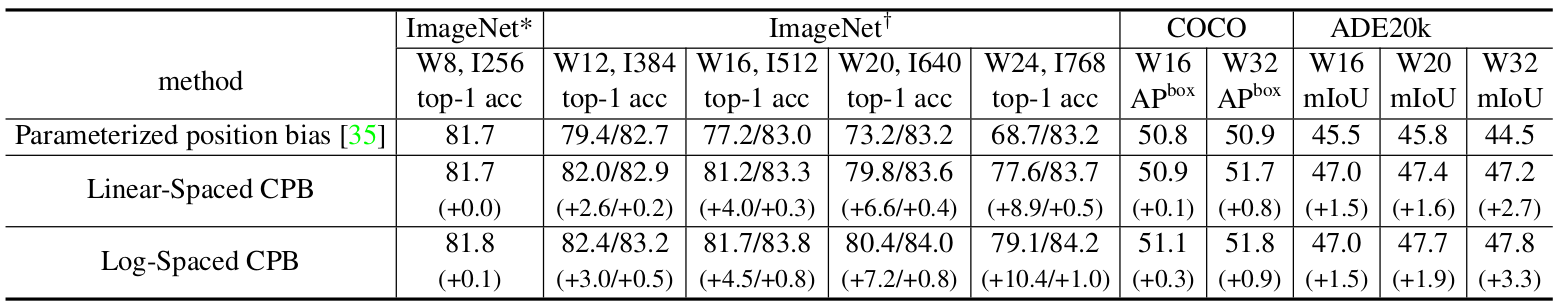
\includegraphics[width=1\columnwidth]{4.png}
        \caption{So sánh các phương pháp tính toán chệch vị khác nhau sử dụng Swin-T. Dấu (*) là để đề cập tới độ chính xác $top-2$ trên tập ImageNet-1k được huấn luyện từ đầu. Các mô hình trong cột (*) sẽ được sử dụng để đánh giá trên các nhiệm vụ phân loại ảnh của tập ImageNet-1K sử dụng độ phân giải của khẩu độ/ảnh lớn hơn, đánh dấu bởi dấu (+). Với các kết quả này, chúng tôi ghi lại cả các kết quả có và không có tinh chỉnh. Các mô hình này cũng được sử dụng cho tinh chỉnh trên các bài toán phát hiện vật thể trên tập COCO và bài toán phân đoạn ngữ nghĩa trên tập ADE20K.}
    \end{table}

    \vspace{5mm}

    \begin{table}[!ht]
        \centering
        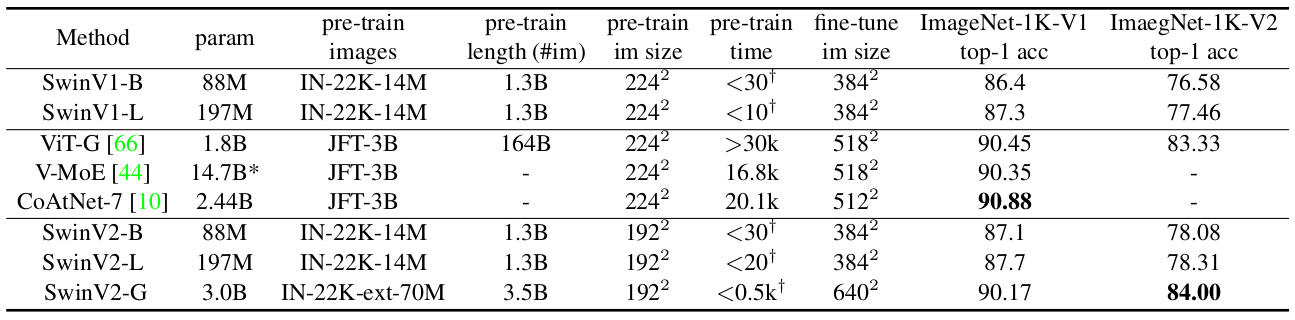
\includegraphics[width=1\columnwidth]{table2.png}
        \caption{So sánh với các mô hình thị giác lớn nhất trước đây trên tập ImageNet-1K V1 và V2. Ký tự * để mô tả đây là mô hình thưa, cột "pre-train time" được đo đạc bởi TPUv3 nhiều ngày với số liệu được lấy từ bài báo gốc. Ký tự \dag của SwinV2-G được ước lượng theo các vòng lặp và FLOPs khi huấn luyện.}
    \end{table}

    \begin{table}
        \parbox{.45\linewidth}{
            \centering
            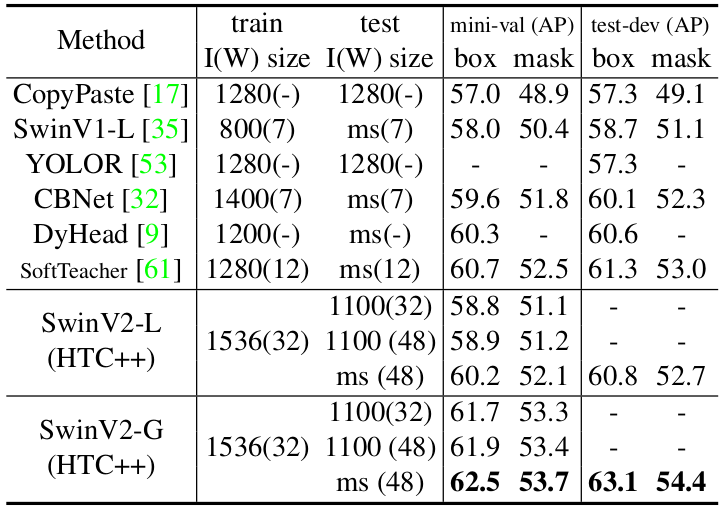
\includegraphics[width=0.45\columnwidth]{table3.png}
            \caption{So sánh với các kết quả tốt nhất trước đây trên tập phân loại và phát hiện vật thể COCO. I(W) là ảnh và kích thước khẩu độ, \textit{ms} nghĩa là thử nghiệm trên nhiều độ phân giải đã được tiến hành.}
        }
        \hfill
        \parbox{.45\linewidth}{
            \centering
            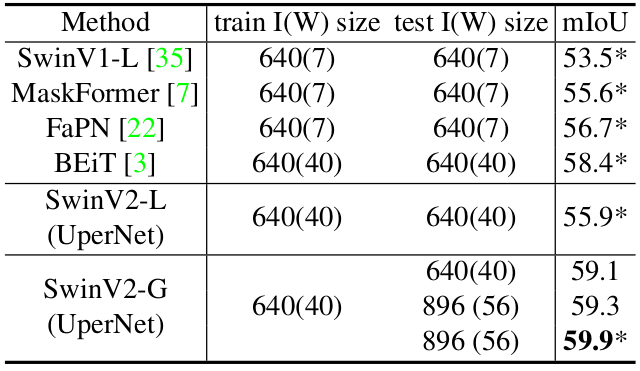
\includegraphics[width=0.45\columnwidth]{table4.png}
            \caption{So sánh với các kết quả tốt nhất trước đây trên tập ADE20K. Ký hiệu * để ám chỉ kiểm thử multi-scale được sử dụng.}
        }
        \vspace{10mm}
    \end{table}

\end{onecolumn}

\twocolumn

\begin{itemize}
    \item Bài toán phát hiện vật thể. COCO được sử dụng để đánh giá. Với các thí nghiệm cho mô hình lớn nhất, chúng tôi tiến hành một bước tiền huấn luyện việc phát hiện vật thể sử dụng tập dữ liệu Object 365 v2, ở giữa bước tiền huấn luyện cho phân loại hình ảnh và bước tinh chỉnh trên tập COCO.
    \item Semantic segmentation. Tập dữ liệu ADE20K được sử dụng.
    \item Phân loại hành động từ video. Tập Kinetics-400 (K400) được sử dụng để đánh giá.
\end{itemize}

% Các thiết lập về tinh chỉnh và tiền huấn luyện sẽ được đề cập chi tiết trong phần phụ lục.

\subsection*{4.2. Mở rộng các thí nghiệm}

Chúng tôi trước hết trình bày về các kết quả trên các đánh giá trực quan bằng việc tăng kích thước của mô hình tới $3$ tỷ tham số và độ phân giải cao cho khẩu độ/ảnh.

Các thiết lập cho thí nghiệm với mô hình SwinV2-G.  Chúng tôi sử dụng độ phân giải nhỏ hơn cho ảnh với kích thươc $192\times192$ pixel trong bước tiền huấn luyện để tiết kiệm chi phí huấn luyện. Chúng tôi tiến hành tiền huấn luyện theo 2 bước. Đầu tiên, mô hình được tiền huấn luyện sử dụng một phương pháp tự giám sát trên tập dữ liệu mở rộng ImageNet-22K-ext với $20$ epochs. Sau đó, mô hình được tiền huấn luyện với $30$ epochs sử dụng bài toán phân loại hình ảnh trên tập dữ liệu này.
% Các thiết lập về tinh chỉnh và tiền huấn luyện sẽ được mô tả trong phần phụ lục.

Trong các phần tiếp theo, chúng tôi trình bày về độ chính xác của SwinV2-G trên các thang đánh giá thị giác tiêu biểu. Lưu ý rằng vì mục đích chính của chúng tôi là để tìm ra làm thế nào để dễ dàng mở rộng năng lực của mô hình và độ phân giải khẩu độ, và liệu các bài toán về thị giác có được lợi ích từ năng lực lớn hơn này không, chúng tôi không so sánh riêng về độ phức tạp hoặc dữ liệu tiền huấn luyện ở đây.

Các kết quả của bài toán phân loại hình ảnh trên tập ImageNet-1K. Bảng 2 so sánh SwinV2-G với các mô hình thị giác tốt nhất trước đây trên ImageNet-1K V1 và V2. SwinV2-G là mô hình thị giác lớn nhất trong số này. Nó đạt độ chính xác top-1 $84\%$ trên đánh giá ImageNet V2, $0.7\%$ cao hơn mô hình tốt nhất trước đây ($83.3\%$). Chúng tôi đạt độ chính chỉ thấp hơn một chút trên tập ImageNet-1K V1 ($90.17\%$ so với $90.88\%$). Sự khác biệt có thể đến từ mức độ tinh chỉnh khác nhau trên tập dữ liệu. Lưu ý rằng, chúng tôi cũng sử dụng ít vòng lặp huấn luyện hơn nhiều và độ phân giải cũng thấp hơn so với các mô hình trước đây, trong khi vẫn cho kết quả rất tốt.

Chúng tôi cũng tiến hành so sánh SwinV2-B và SwinV2-L với mô hình gốc SwinV1-B và SwinV1-L, và thấy tương ứng có sự cải thiện lần lượt $0.8\%$ và $0.4\%$. Sự cải thiện nhỏ hơn ở SwinV2-L so với SwinV2-B ám chỉ rằng nếu vượt quá kích thước này, thì cần nhiều dữ liệu hơn, chính quy hóa (\textit{regularization}) mạnh hơn, hoặc các phương pháp học tự giám sát cao cấp hơn cần được áp dụng.

Kết quả phát hiện vật thể trên tập COCO. Bảng 3 so sánh SwinV2-G với các kết quả tốt nhất trước đây trên bài toán phát hiện vật thể và phân đoạn ngữ nghĩa của tập dữ liệu COCO. Nó đạt kết quả $63.1/54.4$ box/max AP trên tập test-dev của COCO, với tương ứng $+1.8/1.4$ cao hơn các kết quả tốt nhất trước đây ($61.3/53.0$). Điều này chỉ ra rằng việc tăng kích cỡ của mô hình thị giác là có ích cho các bài toán nhận diện thị giác hoặc phát hiện vật thể. Hướng tiếp cận của chúng tôi có thể sử dụng kích thước khẩu độ khác để kiểm tra các ích lợi gia tăng, có thể đóng góp một cách hiệu quả tới hướng tiếp cận Log-Spaced CPB.

Các kết quả semantic segmentation trên tập ADE20K. Bảng 4 so sánh SwinV2-G với các kết quả tốt nhất trước đây trên tập đánh giá ADE20K. Mô hình đã đạt được độ chính xác $59.9 mIoU$ trên tập val ADE20K,  cao hơn $1.5$ so với kết quả tốt nhất trước đây ($58.4$). Điều này chỉ ra rằng việc tăng kích thước mô hình thị giác là có ích cho các bài toán nhận diện thị giác mức độ pixel. Sử dụng kích thước khẩu độ lớn hơn lúc đánh giá có thể tăng thêm $0.2$ độ chính xác, có thể đóng góp tới hướng tiếp cận Log-Spaced CPB.

Các kết quả phân loại hành động từ video trên tập Kinetics-400. Bảng 5 so sánh SwinV2-G với các mô hình tốt nhất trước đây trên tập đánh giá phân loại hành động Kinetics-400. Mô hình đạt được độ chính xác $86.8\%$ top-1, $+1.4\%$ cao hơn kết quả tốt nhất. Điều này chỉ ra rằng việc tăng kích thước mô hình thị giác cũng đem lại ích lợi cho các bài toán nhận diện video. Trong ngữ cảnh này, sử dụng kích thước khẩu độ lớn hơn lúc đánh giá có thể đem lại $+0.2\%$ độ chính xác, có thể đóng góp tới hướng tiếp cận Log-Spaced CPB.


\begin{table}[!ht]
    \centering
    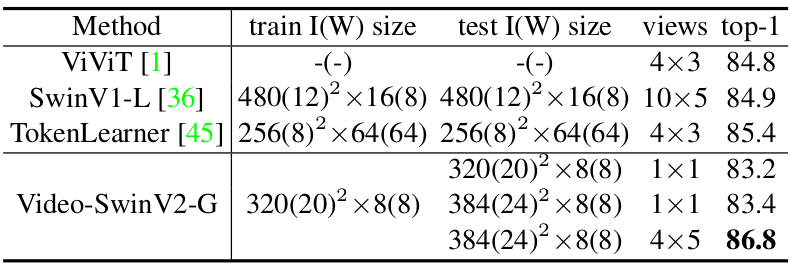
\includegraphics[width=1\columnwidth]{table5.png}
    \caption{So sánh với các kết quả tốt nhất trên dữ liệu phân loại hành động trên video Kinetics-400.}
\end{table}

\begin{table}[!ht]
    \centering
    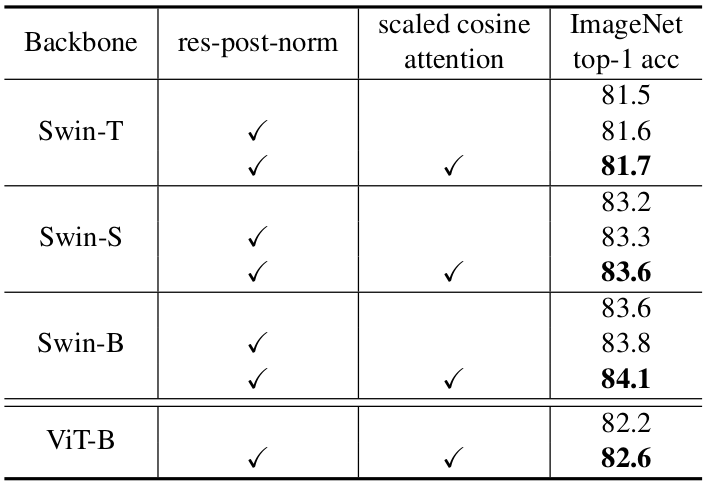
\includegraphics[width=1\columnwidth]{table6.png}
    \caption{Lược bỏ tiến hành trên lớp res-post-norm và cosine attention.}
\end{table}

\begin{table}[!ht]
    \centering
    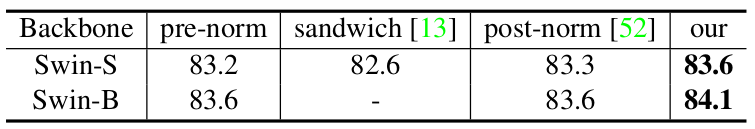
\includegraphics[width=1\columnwidth]{table7.png}
    \caption{So sánh với các phương pháp chuẩn hóa khác. Phương pháp post-norm phân kỳ ở learning rate mặc định, và chúng tôi sử dụng 1/4 giá trị learning rate mặc định cho phương pháp này. Sandwich cho kết quả kém hơn kết quả của chúng tôi.}
\end{table}

\begin{table}[!ht]
    \centering
    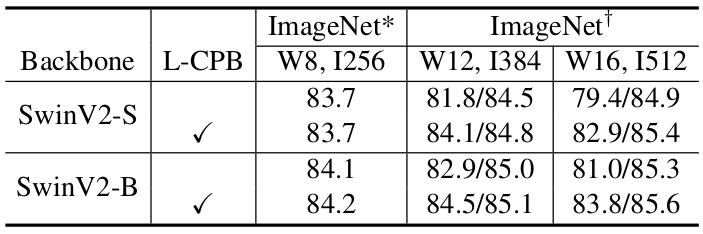
\includegraphics[width=1\columnwidth]{table8.png}
    \caption{Lược bỏ trên Log-CPB sử dụng các kích thước mô hình khác nhau.}
\end{table}

\subsection*{4.3. Các nghiên cứu về việc lược bỏ:}
Lược bỏ phần về cụm các lớp res-post-norm và tập trung cosin mở rộng \textit{scaled cosin attention}: Bảng 6 lược bỏ phần hiệu năng cho đề xuất cụm các lớp res-post-norm và \textit{scaled cosin attention} cho mô hình Swin Transformer. Cả 2 kỹ thuật đều cải thiện độ chính xác cho các kích thước rất nhỏ, nhỏ và gốc, tương ứng là $+0.2\%$, $+0.4\%$ và $+0.5\%$, thêm vào đó, các kỹ thuật này cũng có ích lợi với các mô hình lớn hơn. Ví dụ như nó cũng có ích với kiến trúc ViT ($+0.4\%$). Hướng chuẩn hóa được đề xuất cũng tốt hơn một số cách chuẩn hóa khác, như được trình bày trong Bảng 7.

Quan trọng hơn, việc kết hợp post-norm và \textit{scaled cosine attention} giúp ổn định quá trình huấn luyện. Như được trình bày trong bảng 2, trong khi các giá trị kích hoạt ở các lớp sâu hơn ở mô hình Swin Transformer gốc trở nên rất lớn ở kích thước lớn, mô hình phiên bản mới này cho thấy tác động nhẹ hơn nhiều. Với mô hình kích thước rất lớn, việc tiền huấn luyện tự giám sát bị phân kỳ khi sử dụng mô hình Swin Transformer gốc, trong khi huấn luyện tốt trên mô hình Swin Transformer V2.

Tăng độ phân giải khẩu độ bằng các hướng tiếp cận khác: Bảng 1 và 8 loại bỏ phần hiệu năng của $3$ cách tiếp cận bằng cách tăng độ phân giải khẩu độ từ $256\times256$ lúc tiền huấn luyện tới các kích thước lớn hơn trong $3$ bài toán phân loại hình ảnh trên tập ImageNet-1K, nhận diện vật thể COCO, và semantic segmentation ADE20K. Có thể thấy rằng:
\begin{itemize}
    \item 1) Các hướng tiếp cận khác nhau cho kết quả tương tự nhau ở bước tiền huấn luyện ($81.7\%-81.8\%$)
    \item 2) Khi chuyển đổi tới các bài toán down-stream, hướng tiếp cận bias vị trí tương đối liên tục (CPB) thể hiện tốt hơn hướng tiếp cận bias được tham số hóa sử dụng trong Swin Transformer V1. So sánh với cách tiếp cận không gian tuyến tính, phiên bản không gian log tốt hơn một chút.
    \item 3) Thay đổi càng lớn về độ phân giải giữa tiền huấn luyện và bước tinh chỉnh, thì hướng tiếp cận CPB log-spaced cho lợi ích càng lớn.
\end{itemize}

Trong Bảng 1 và Bảng 8, chúng tôi cũng trình bày về độ chính xác sử dụng độ phân giải khẩu độ đích mà không cần tinh chỉnh (fine-tuning) (xem con số đầu tiên trong mỗi cột ở thí nghiệm trên tập ImageNet-1K). Độ chính xác nhận diện vẫn không kém ngay cả khi kích thước khẩu độ tăng từ $8$ tới $24$ ($78.9\%$ so với $81.8\%$), trong khi độ chính xác $top-1$ accuracy của hướng tiếp cận ban đầu giảm đáng kể từ $81.7\%$ xuống $68.7\%$. Cũng lưu ý rằng khi không có tinh chỉnh, sử dụng kích thước khẩu độ $12$ mà mô hình tiền huấn luyện chưa thấy trước đó có thể đem lại độ chính xác tăng thêm $+0.4\%$ so với độ chính xác ban đầu. Điều này chỉ ra rằng chúng ta có thể cải thiện độ chính xác thông qua việc điều chỉnh khẩu độ lúc đánh giá, như được quan sát trong Bảng 3,4, và 5.

\section*{5. Kết luận}
Chúng tôi và trình bày các kỹ thuật cho việc tăng kích thước của mô hình Swin Transformer lên tới $3$ tỷ tham số và giúp mô hình có khả năng huấn luyện được với kích cỡ ảnh lên tới $1,536 \times 1,536$ pixel, bao gồm các kỹ thuật res-post-norm và \textit{scaled cosine attention} để giúp dễ dàng hơn tăng năng lực của mô hình, cũng như hướng tiếp cận chệch vị tương đối liên tục không gian log để giúp mô hình hiệu quả hơn khi thay đổi độ phân giải của khẩu độ. Kiến trúc mới này được đặt tên là Swin Transformer V2, và bằng việc tăng năng lực và độ phân giải của mô hình, nó đã đạt kỷ lục mới về độ chính xác trên cả 4 đánh giá đại diện cho các bài toán về thị giác. Nhờ những kết quả mạnh mẽ này, chúng tôi kỳ vọng sẽ tiến hành nhiều nghiên cứu nữa theo hướng này để có thể tiệm cận được năng lực xử lý của các mô hình ngôn ngữ và tạo điều kiện cho việc mô hình hóa liên hợp giữa 2 lĩnh vực thị giác và ngôn ngữ.

\section*{Lời cảm ơn}
Chúng tôi cảm ơn các đồng nghiệp ở Microsoft nói chung, và Eric Chang, Lidong Zhou, Jing Tao, Aaron Zhang, Edward Cui, Bin Xiao, Lu Yuan, Peng Cheng, Fan Yang nói riêng về những thảo luận hữu ích cũng như sự giúp đỡ nhiệt tình về tài nguyên GPU và dữ liệu.

% \section*{Tham khảo}

% \begin{thebibliography}{1}
%     \bibitem{1} Anurag Arnab, Mostafa Dehghani, Georg Heigold, Chen Sun, Mario Lučić, and Cordelia Schmid. Vivit: A video vision transformer, 2021. 3, 7
%     \bibitem{2} Jimmy Lei Ba, Jamie Ryan Kiros, and Geoffrey E. Hinton. Layer normalization, 2016. 3
%     \bibitem{3} Hangbo Bao, Li Dong, and Furu Wei. Beit: Bert pre-training of image transformers, 2021. 2, 7
%     \bibitem{4} Andrew Brock, Soham De, and Samuel L Smith. Characterizing signal propagation to close the performance gap in unnormalized resnets. arXiv preprint arXiv:2101.08692, 2021. 4
%     \bibitem{5} Tom B. Brown, Benjamin Mann, Nick Ryder, Melanie Subbiah, Jared Kaplan, Prafulla Dhariwal, Arvind Neelakantan, Pranav Shyam, Girish Sastry, Amanda Askell, Sandhini Agarwal, Ariel Herbert-Voss, Gretchen Krueger, Tom Henighan, Rewon Child, Aditya Ramesh, Daniel M. Ziegler, Jeffrey Wu, Clemens Winter, Christopher Hesse, Mark Chen, Eric Sigler, Mateusz Litwin, Scott Gray, Benjamin Chess, Jack Clark, Christopher Berner, Sam McCandlish, Alec Radford, Ilya Sutskever, and Dario Amodei. Language models are few-shot learners, 2020. 1, 2
%     \bibitem{6} TianqiChen,BingXu,ChiyuanZhang,andCarlosGuestrin. Training deep nets with sublinear memory cost, 2016. 2, 6
%     \bibitem{7} Bowen Cheng, Alexander G. Schwing, and Alexander Kir- illov. Per-pixel classification is not all you need for semantic segmentation. arXiv, 2021. 7
%     \bibitem{8} Xiangxiang Chu, Zhi Tian, Yuqing Wang, Bo Zhang, Haib- ing Ren, Xiaolin Wei, Huaxia Xia, and Chunhua Shen. Twins: Revisiting the design of spatial attention in vision transformers, 2021. 3
%     \bibitem{9} Xiyang Dai, Yinpeng Chen, Bin Xiao, Dongdong Chen, Mengchen Liu, Lu Yuan, and Lei Zhang. Dynamic head: Unifying object detection heads with attentions, 2021. 7
%     \bibitem{10} Zihang Dai, Hanxiao Liu, Quoc V. Le, and Mingxing Tan. Coatnet: Marrying convolution and attention for all data sizes, 2021. 2, 3, 5, 7
%     \bibitem{11} Jia Deng, Wei Dong, Richard Socher, Li-Jia Li, Kai Li, and Li Fei-Fei. Imagenet: A large-scale hierarchical image database. In 2009 IEEE conference on computer vision and pattern recognition, pages 248–255. Ieee, 2009. 6
%     \bibitem{12} Jacob Devlin, Ming-Wei Chang, Kenton Lee, and Kristina Toutanova. Bert: Pre-training of deep bidirectional transformers for language understanding. arXiv preprint arXiv:1810.04805, 2018. 1, 2
%     \bibitem{13} Ming Ding, Zhuoyi Yang, Wenyi Hong, Wendi Zheng, Chang Zhou, Da Yin, Junyang Lin, Xu Zou, Zhou Shao, Hongxia Yang, and Jie Tang. Cogview: Mastering text- to-image generation via transformers. arXiv preprint arXiv:2105.13290, 2021. 3, 8
%     \bibitem{14} Xiaoyi Dong, Jianmin Bao, Dongdong Chen, Weiming Zhang, Nenghai Yu, Lu Yuan, Dong Chen, and Baining Guo. Cswin transformer: A general vision transformer backbone with cross-shaped windows, 2021. 3
%     \bibitem{15} Alexey Dosovitskiy, Lucas Beyer, Alexander Kolesnikov, Dirk Weissenborn, Xiaohua Zhai, Thomas Unterthiner, Mostafa Dehghani, Matthias Minderer, Georg Heigold, Syl- vain Gelly, Jakob Uszkoreit, and Neil Houlsby. An image is worth 16x16 words: Transformers for image recognition at scale. In International Conference on Learning Representa- tions, 2021. 2, 3
%     \bibitem{16} William Fedus, Barret Zoph, and Noam Shazeer. Switch transformers: Scaling to trillion parameter models with simple and efficient sparsity, 2021. 1, 2
%     \bibitem{17} Golnaz Ghiasi, Yin Cui, Aravind Srinivas, Rui Qian, Tsung- Yi Lin, Ekin D Cubuk, Quoc V Le, and Barret Zoph. Simple copy-paste is a strong data augmentation method for instance segmentation. arXiv preprint arXiv:2012.07177, 2020. 7
%     \bibitem{18} PriyaGoyal,MathildeCaron,BenjaminLefaudeux,MinXu, Pengchao Wang, Vivek Pai, Mannat Singh, Vitaliy Liptchin- sky, Ishan Misra, Armand Joulin, and Piotr Bojanowski. Self-supervised pretraining of visual features in the wild, 2021. 2
%     \bibitem{19} Kaiming He, Xiangyu Zhang, Shaoqing Ren, and Jian Sun. Deep residual learning for image recognition. In Proceedings of the IEEE conference on computer vision and pattern recognition, pages 770–778, 2016. 1
%     \bibitem{20} Han Hu, Jiayuan Gu, Zheng Zhang, Jifeng Dai, and Yichen Wei. Relation networks for object detection. In Proceed- ings of the IEEE Conference on Computer Vision and Pattern Recognition, pages 3588–3597, 2018. 3
%     \bibitem{21} Han Hu, Zheng Zhang, Zhenda Xie, and Stephen Lin. Local relation networks for image recognition. In Proceedings of the IEEE/CVF International Conference on Computer Vision (ICCV), pages 3464–3473, October 2019. 3
%     \bibitem{22} Shihua Huang, Zhichao Lu, Ran Cheng, and Cheng He. Fapn: Feature-aligned pyramid network for dense image prediction, 2021. 7
%     \bibitem{23} Zilong Huang, Youcheng Ben, Guozhong Luo, Pei Cheng, Gang Yu, and Bin Fu. Shuffle transformer: Rethinking spatial shuffle for vision transformer, 2021. 3
%     \bibitem{24} Sergey Ioffe and Christian Szegedy. Batch normalization: Accelerating deep network training by reducing internal covariate shift, 2015. 3
%     \bibitem{25} Jared Kaplan, Sam McCandlish, Tom Henighan, Tom B. Brown, Benjamin Chess, Rewon Child, Scott Gray, Alec Radford, Jeffrey Wu, and Dario Amodei. Scaling laws for neural language models, 2020. 2
%     \bibitem{26} Will Kay, Joao Carreira, Karen Simonyan, Brian Zhang, Chloe Hillier, Sudheendra Vijayanarasimhan, Fabio Viola, Tim Green, Trevor Back, Paul Natsev, et al. The kinetics hu- man action video dataset. arXiv preprint arXiv:1705.06950, 2017. 6
%     \bibitem{27} Guolin Ke, Di He, and Tie-Yan Liu. Rethinking positional encoding in language pre-training, 2021. 3
%     \bibitem{28} Alexander Kolesnikov, Lucas Beyer, Xiaohua Zhai, Joan Puigcerver, Jessica Yung, Sylvain Gelly, and Neil Houlsby. Big transfer (bit): General visual representation learning. arXiv preprint arXiv:1912.11370, 6(2):8, 2019. 2
%     \bibitem{29} Alex Krizhevsky, Ilya Sutskever, and Geoffrey E Hinton. Imagenet classification with deep convolutional neural networks. In Advances in neural information processing sys- tems, pages 1097–1105, 2012. 2
%     \bibitem{30} Yann LeCun, Le ́on Bottou, Yoshua Bengio, Patrick Haffner, et al. Gradient-based learning applied to document recognition. Proceedings of the IEEE, 86(11):2278–2324, 1998. 2
%     \bibitem{31} Yawei Li, Kai Zhang, Jiezhang Cao, Radu Timofte, and Luc Van Gool. Localvit: Bringing locality to vision trans- formers, 2021. 3
%     \bibitem{32} Tingting Liang, Xiaojie Chu, Yudong Liu, Yongtao Wang, Zhi Tang, Wei Chu, Jingdong Chen, and Haibin Ling. Cb- netv2: A composite backbone network architecture for ob- ject detection, 2021. 7
%     \bibitem{33} Tsung-Yi Lin, Michael Maire, Serge Belongie, James Hays, Pietro Perona, Deva Ramanan, Piotr Dolla ́r, and C Lawrence Zitnick. Microsoft coco: Common objects in context. In European conference on computer vision, pages 740–755. Springer, 2014. 6
%     \bibitem{34} Ze Liu, Han Hu, Yue Cao, Zheng Zhang, and Xin Tong. A closer look at local aggregation operators in point cloud analysis, 2020. 3
%     \bibitem{abc} Ze Liu, Yutong Lin, Yue Cao, Han Hu, Yixuan Wei, Zheng Zhang, Stephen Lin, and Baining Guo. Swin trans- former: Hierarchical vision transformer using shifted win- dows, 2021. 1, 2, 3, 5, 7
%     \bibitem{36} Ze Liu, Jia Ning, Yue Cao, Yixuan Wei, Zheng Zhang, Stephen Lin, and Han Hu. Video swin transformer, 2021. 2,7
%     \bibitem{37} Microsoft. Turing-nlg: A 17-billion-parameter language model by microsoft, 2020. 1, 2
%     \bibitem{38} Microsoft. Using deepspeed and megatron to train megatron-turing nlg 530b, the world’s largest and most powerful generative language model, 2021. 1, 2
%     \bibitem{39} Alec Radford, Jong Wook Kim, Chris Hallacy, Aditya Ramesh, Gabriel Goh, Sandhini Agarwal, Girish Sastry, Amanda Askell, Pamela Mishkin, Jack Clark, Gretchen Krueger, and Ilya Sutskever. Learning transferable visual models from natural language supervision, 2021. 6
%     \bibitem{40} Alec Radford, Jeff Wu, Rewon Child, David Luan, Dario Amodei, and Ilya Sutskever. Language models are unsuper-
%     vised multitask learners. 2019. 1, 2, 3
%     \bibitem{41} olin Raffel, Noam Shazeer, Adam Roberts, Katherine Lee, Sharan Narang, Michael Matena, Yanqi Zhou, Wei Li, and Peter J. Liu. Exploring the limits of transfer learning with a unified text-to-text transformer. Journal of Machine Learn- ing Research, 21(140):1–67, 2020. 1, 2, 3
%     \bibitem{42} Samyam Rajbhandari, Jeff Rasley, Olatunji Ruwase, and Yuxiong He. Zero: Memory optimizations toward training trillion parameter models, 2020. 2, 5
%     \bibitem{43} Benjamin Recht, Rebecca Roelofs, Ludwig Schmidt, and Vaishaal Shankar. Do imagenet classifiers generalize to im- agenet?, 2019. 2, 6, 7
%     \bibitem{44} Carlos Riquelme, Joan Puigcerver, Basil Mustafa, Maxim Neumann, Rodolphe Jenatton, Andre ́ Susano Pinto, Daniel
%     Keysers, and Neil Houlsby. Scaling vision with sparse mix-ture of experts, 2021. 2, 3, 5, 7
%     \bibitem{45} Michael S. Ryoo, AJ Piergiovanni, Anurag Arnab, Mostafa Dehghani, and Anelia Angelova. Tokenlearner: What can 8 learned tokens do for images and videos?, 2021. 2, 7, 8
%     \bibitem{46} Kristof T Schu ̈tt, Pieter-Jan Kindermans, Huziel E Sauceda, Stefan Chmiela, Alexandre Tkatchenko, and Klaus-Robert Mu ̈ller. Schnet: A continuous-filter convolutional neural network for modeling quantum interactions. arXiv preprint arXiv:1706.08566, 2017. 3
%     \bibitem{47} Shuai Shao, Zeming Li, Tianyuan Zhang, Chao Peng, Gang Yu, Xiangyu Zhang, Jing Li, and Jian Sun. Objects365: A large-scale, high-quality dataset for object detection. In Proceedings of the IEEE/CVF International Conference on Computer Vision (ICCV), October 2019. 6
%     \bibitem{48} K. Simonyan and A. Zisserman. Very deep convolutional networks for large-scale image recognition. In International Conference on Learning Representations, May 2015. 1, 2
%     \bibitem{49} Christian Szegedy, Wei Liu, Yangqing Jia, Pierre Sermanet, Scott Reed, Dragomir Anguelov, Dumitru Erhan, Vincent Vanhoucke, and Andrew Rabinovich. Going deeper with convolutions. In Proceedings of the IEEE conference on computer vision and pattern recognition, pages 1–9, 2015.  2
%     \bibitem{50} Hugo Touvron, Matthieu Cord, Matthijs Douze, Francisco Massa, Alexandre Sablayrolles, and Herve ́ Je ́gou. Training data-efficient image transformers & distillation through at- tention. arXiv preprint arXiv:2012.12877, 2020. 3
%     \bibitem{51} Dmitry Ulyanov, Andrea Vedaldi, and Victor Lempitsky. In- stance normalization: The missing ingredient for fast styliza- tion, 2017. 3
%     \bibitem{52} Ashish Vaswani, Noam Shazeer, Niki Parmar, Jakob Uszko- reit, Llion Jones, Aidan N Gomez, Łukasz Kaiser, and Illia Polosukhin. Attention is all you need. In Advances in Neural Information Processing Systems, pages 5998–6008, 2017. 2, 3,8
%     \bibitem{53} Chien-Yao Wang, I-Hau Yeh, and Hong-Yuan Mark Liao. You only learn one representation: Unified network for mul- tiple tasks, 2021. 7
%     \bibitem{54} Shenlong Wang, Simon Suo, Wei-Chiu Ma, Andrei Pokrovsky, and Raquel Urtasun. Deep parametric continu- ous convolutional neural networks. 2018 IEEE/CVF Confer- ence on Computer Vision and Pattern Recognition, Jun 2018. 3
%     \bibitem{55} Wenhai Wang, Enze Xie, Xiang Li, Deng-Ping Fan, Kaitao Song, Ding Liang, Tong Lu, Ping Luo, and Ling Shao. Pyra- mid vision transformer: A versatile backbone for dense pre- diction without convolutions, 2021. 3
%     \bibitem{56} Kan Wu, Houwen Peng, Minghao Chen, Jianlong Fu, and Hongyang Chao. Rethinking and improving relative position encoding for vision transformer, 2021. 3
%     \bibitem{57} Yuxin Wu and Kaiming He. Group normalization. In Pro- ceedings of the European Conference on Computer Vision (ECCV), pages 3–19, 2018. 3
%     \bibitem{58} Tete Xiao, Mannat Singh, Eric Mintun, Trevor Darrell, Piotr Dolla ́r, and Ross Girshick. Early convolutions help trans- formers see better. arXiv preprint arXiv:2106.14881, 2021. 3
%     \bibitem{59} Zhenda Xie, Zheng Zhang, Yue Cao, Yutong Lin, Jianmin Bao, Zhuliang Yao, Qi Dai, and Han Hu. Simmim: A sim- ple framework for masked image modeling. In Tech report, 2022.4,5,6,8
%     \bibitem{60} Ruibin Xiong, Yunchang Yang, Di He, Kai Zheng, Shuxin Zheng, Chen Xing, Huishuai Zhang, Yanyan Lan, Liwei Wang, and Tie-Yan Liu. On layer normalization in the trans- former architecture. 2020. 3
%     \bibitem{61} Mengde Xu, Zheng Zhang, Han Hu, Jianfeng Wang, Lijuan Wang, Fangyun Wei, Xiang Bai, and Zicheng Liu. End-to- end semi-supervised object detection with soft teacher, 2021. 2, 7
%     \bibitem{62} JianweiYang,ChunyuanLi,PengchuanZhang,XiyangDai, Bin Xiao, Lu Yuan, and Jianfeng Gao. Focal self-attention for local-global interactions in vision transformers, 2021. 3
%     \bibitem{63} Zhuliang Yao, Yue Cao, Yutong Lin, Ze Liu, Zheng Zhang, and Han Hu. Leveraging batch normalization for vision transformers. In Proceedings of the IEEE/CVF International Conference on Computer Vision, pages 413–422, 2021. 4
%     \bibitem{64} Li Yuan, Yunpeng Chen, Tao Wang, Weihao Yu, Yujun Shi, Zihang Jiang, Francis EH Tay, Jiashi Feng, and Shuicheng Yan. Tokens-to-token vit: Training vision transformers from scratch on imagenet, 2021. 3
%     \bibitem{65} Li Yuan, Qibin Hou, Zihang Jiang, Jiashi Feng, and Shuicheng Yan. Volo: Vision outlooker for visual recog- nition. arXiv preprint arXiv:2106.13112, 2021. 3
%     \bibitem{66} XiaohuaZhai,AlexanderKolesnikov,NeilHoulsby,andLu- cas Beyer. Scaling vision transformers, 2021. 2, 3, 5, 7
%     \bibitem{67} Pengchuan Zhang, Xiyang Dai, Jianwei Yang, Bin Xiao, Lu Yuan, Lei Zhang, and Jianfeng Gao. Multi-scale vision long- former: A new vision transformer for high-resolution image encoding, 2021. 3
%     \bibitem{68} Sixiao Zheng, Jiachen Lu, Hengshuang Zhao, Xiatian Zhu, Zekun Luo, Yabiao Wang, Yanwei Fu, Jianfeng Feng, Tao Xiang, Philip HS Torr, et al. Rethinking semantic segmen- tation from a sequence-to-sequence perspective with trans- formers. arXiv preprint arXiv:2012.15840, 2020. 3
%     \bibitem{69} Bolei Zhou, Hang Zhao, Xavier Puig, Tete Xiao, Sanja Fi- dler, Adela Barriuso, and Antonio Torralba. Semantic under- standing of scenes through the ade20k dataset. International Journal on Computer Vision, 2018. 6
% \end{thebibliography}

\end{document}

